\section{Finding the relative-volatility signal}\label{sec:4}

\subsection*{Relative richness across related names}

For each pair, we compare the IV difference D = IV\_A - IV\_B with its latest 252 trading sessions, requiring 63 observations. At the upper quintile we sell A's relatively high-IV put and buy B's; at the lower quintile we reverse direction. Historical ranking matters: a ten-point gap means something different for a pair usually five points apart than for one usually fifteen points apart.


\begin{figure}[!htbp]\centering
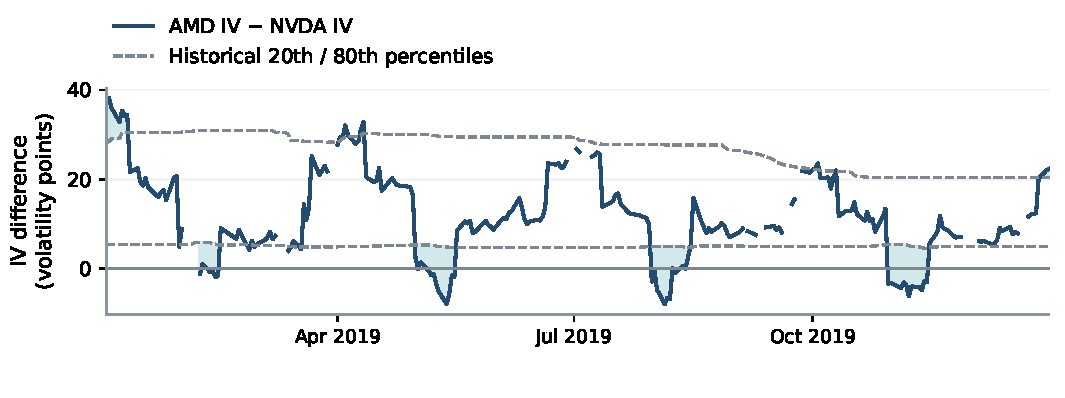
\includegraphics[width=\linewidth]{signal_example.pdf}
\caption{AMD minus NVDA selected-put IV in 2019. Shading marks excursions outside historical percentile boundaries, not executed trades. Gaps are unavailable quotes. Daily contract selection makes this a signal series, not the mark of one held contract.}\label{fig:signal-example}
\end{figure}

Monthly formation requires 126-session return beta between 0.85 and 1.15 and correlation of at least 0.5. The proposed direction must also show positive historical profit per initial vega over 91 and 365 calendar days, with 21 and 63 completed observations. These are simulated standalone candidates, not just funded fills. A trade entered yesterday with a month left cannot contribute its eventual profit today.


\subsection*{Why an extreme is not enough}

Beta measures the scale of one name's response to the other; correlation measures how consistently they move together. Neither guarantees that their option prices should behave alike. The relatedness screens keep the comparison among reasonably similar names without treating relatedness as the trading signal.


The profitability memory adds a different economic question: has this direction recently paid for the premium and hedging costs? We are looking for an unusually wide IV difference in a direction with evidence of structural relative richness, rather than assuming every large gap must revert. The memory and completed-count conditions are selected rules, shared across all put sizing controls.


The chart follows each day's selected contract. After entry, the simulator holds the purchased and sold contracts rather than replacing them when daily selection changes. Profit therefore depends on their realized option and hedge cash flows. A temporary narrowing of the displayed IV gap is neither required nor sufficient for a profitable expiry trade.


\FloatBarrier
